\begin{tikzpicture}[
    every node/.style={node distance=2mm, inner sep=0, outer sep=0},
    image/.style={}
]
    \node[image] (img1){
        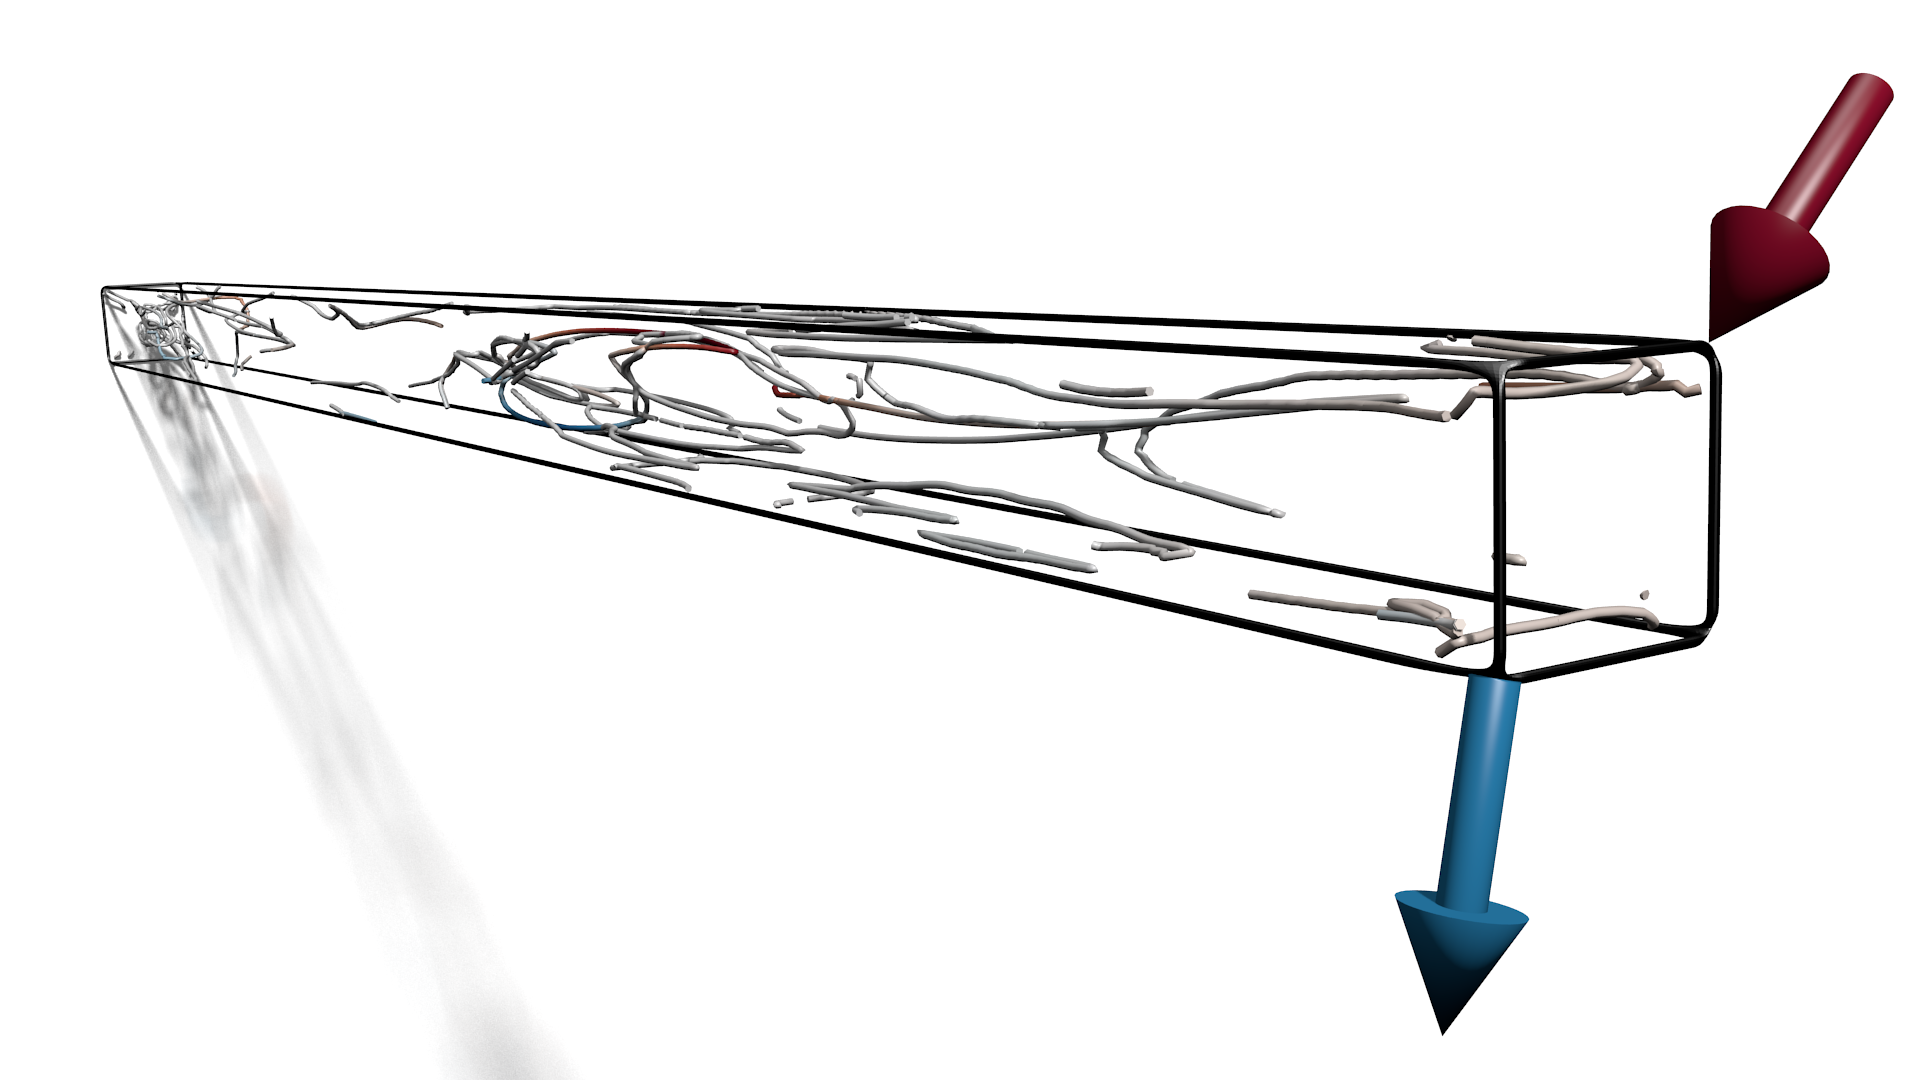
\includegraphics[width=\figurewidth]{figures/beam_full_total}
    };

    \node[image, below=of img1.south west, anchor=north west] (img2) {
        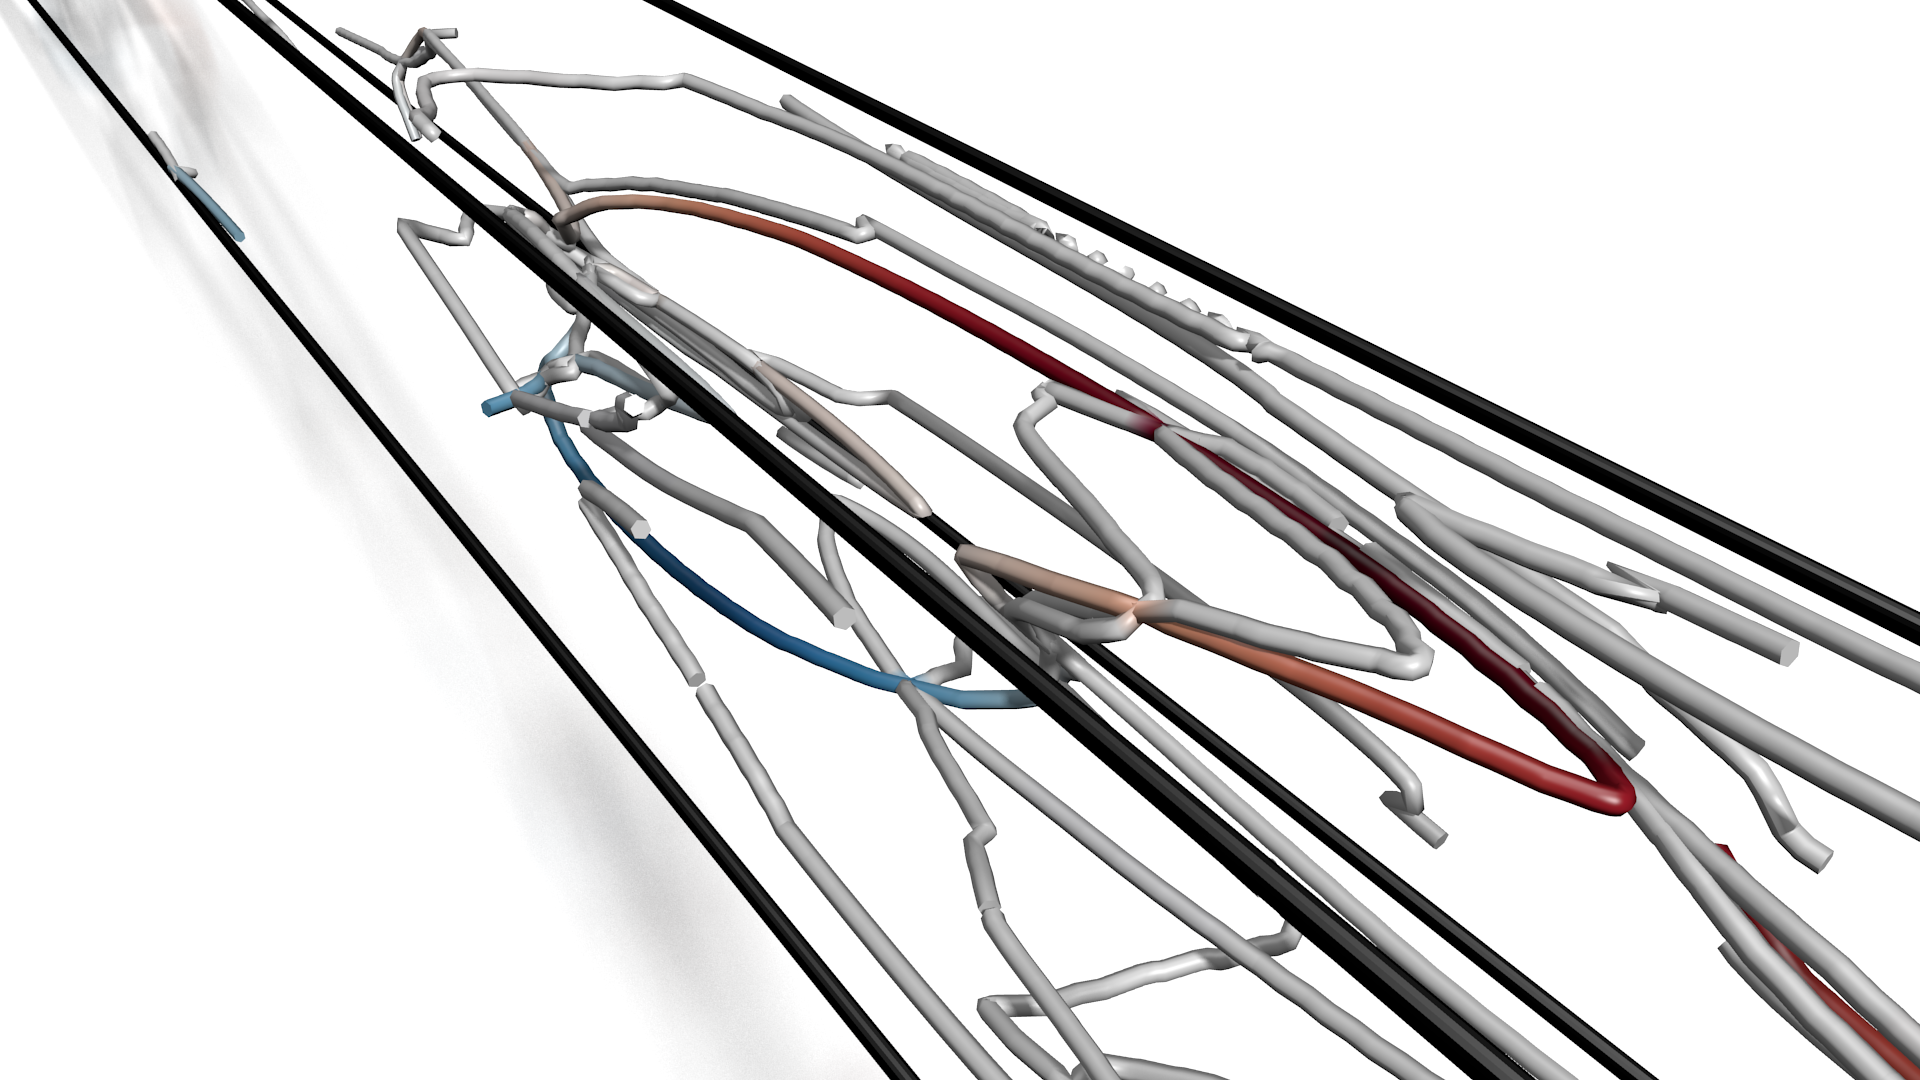
\includegraphics[width=0.5\figurewidth-2mm/2]{figures/beam_full_detail1}
    };
    \begin{scope}[
        shift=(img2.south west), % origin is lower left corner
        x={($(img2.south east)-(img2.south west)$)}, % x axis is lower side
        y={($(img2.north west)-(img2.south west)$)}] % y axis is left side
        % \draw[help lines, opacity=0.5, xstep=.01,ystep=.01] (0,0) grid (1,1);
        % \draw[thin, xstep=.1,ystep=.1] (0,0) grid (1,1);
        % \foreach \x in {0,...,9} { \node [anchor=north] at (\x/10,0) {0.\x}; }
        % \foreach \y in {0,...,9} { \node [anchor=east] at (0,\y/10) {0.\y}; }
        \draw[mycolor4, thick, rotate around={-25:(0.55, 0.5)}]
            (0.55, 0.5) ellipse (0.35 and 0.25);
    \end{scope}

    \node[image, right=of img2] (img4) {
        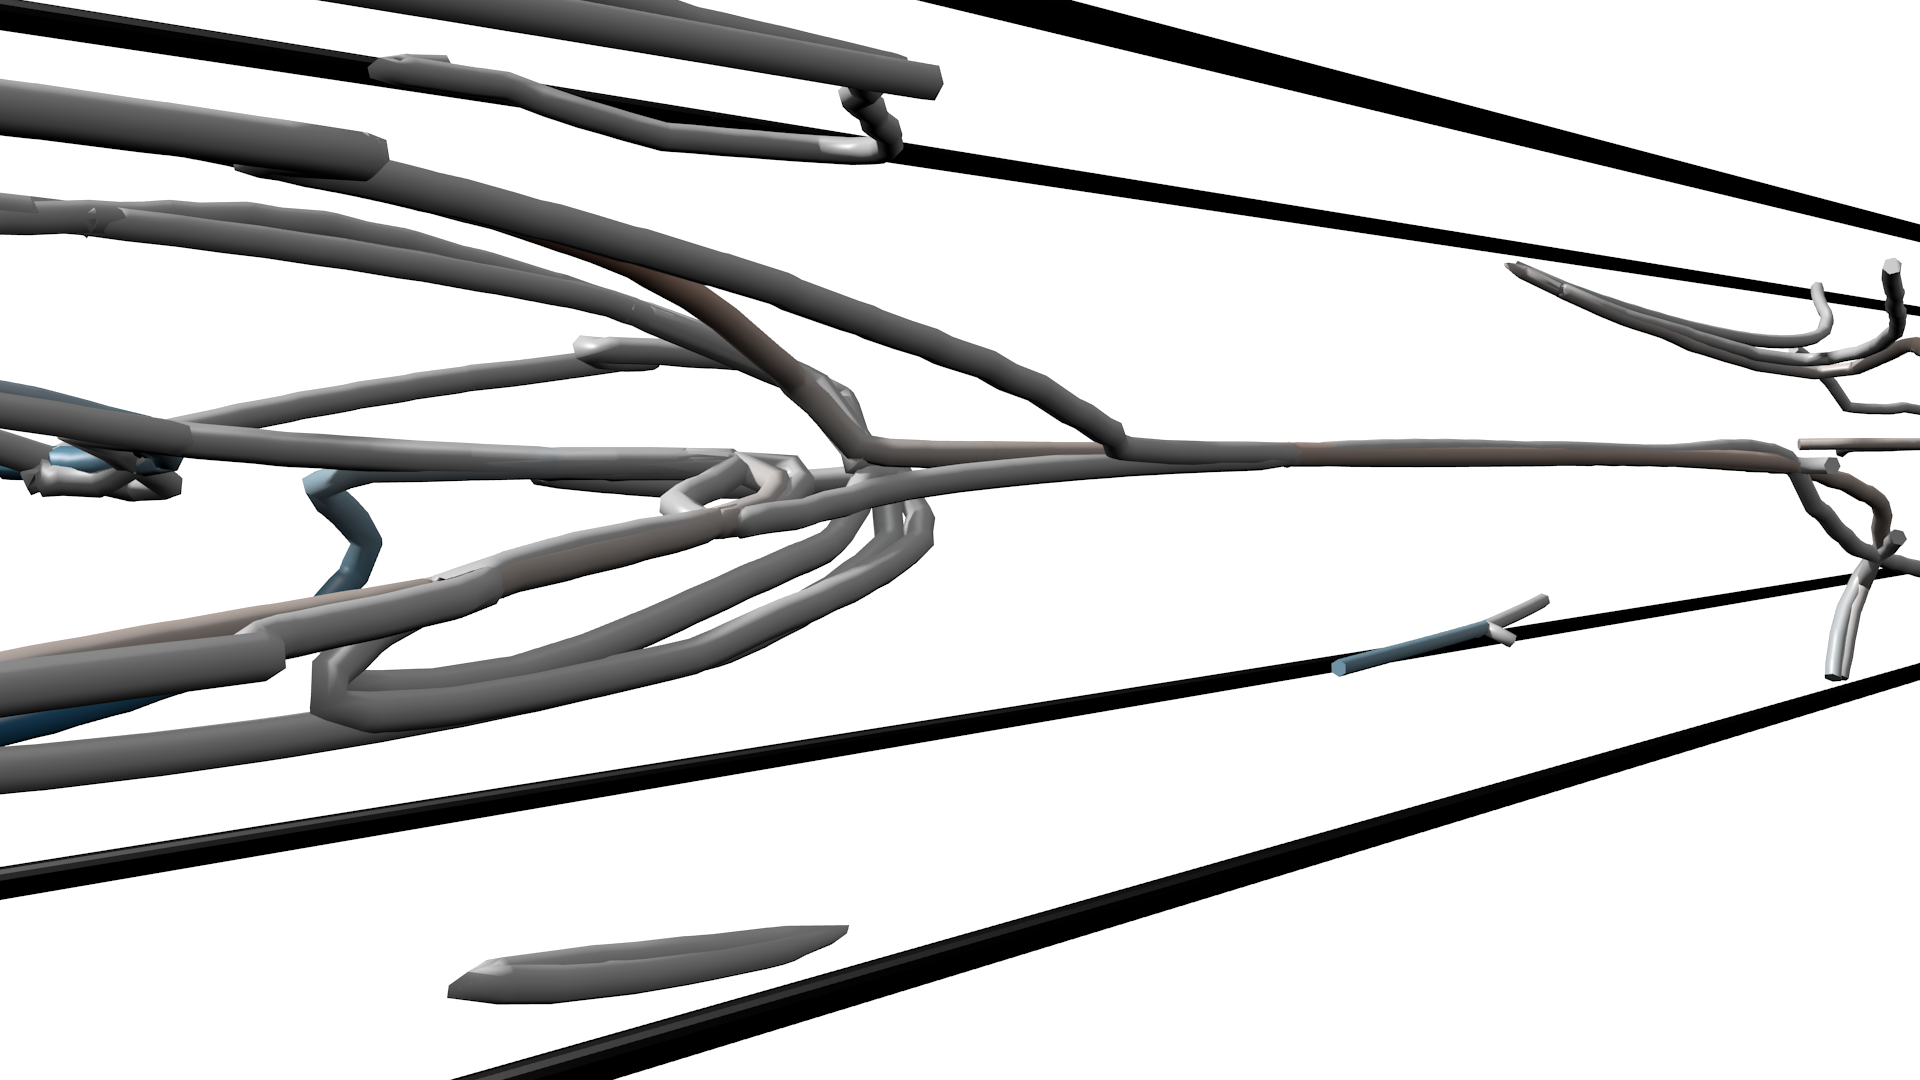
\includegraphics[width=0.5\figurewidth-2mm/2]{figures/beam_full_detail2}
    };
    \begin{scope}[
        shift=(img4.south west), % origin is lower left corner
        x={($(img4.south east)-(img4.south west)$)}, % x axis is lower side
        y={($(img4.north west)-(img4.south west)$)}] % y axis is left side
        % \draw[help lines, opacity=0.5, xstep=.01,ystep=.01] (0,0) grid (1,1);
        % \draw[thin, xstep=.1,ystep=.1] (0,0) grid (1,1);
        % \foreach \x in {0,...,9} { \node [anchor=north] at (\x/10,0) {0.\x}; }
        % \foreach \y in {0,...,9} { \node [anchor=east] at (0,\y/10) {0.\y}; }
        \draw[mycolor4, thick] (0.75, 0.58) ellipse (0.2 and 0.05);
    \end{scope}
\end{tikzpicture}%